\section{MPI parallelisation}
  \label{section:parallelisation:mpi}


\chapterDescription
  {
    180 minutes.
  }
  {
    A working simulation code and working MPI environment.
  }

In this section, we discuss how to parallelise a simulation code with message
passing.

\subsection{Preparation}

Peano technically relies on MPI with its SPMD paradigm, i.e.~all ranks run
exactly the same code.
Internally, it however creates a logical tree topology on all ranks and
reserves one rank for non-compute tasks.
This one is called the {\em global master}.
By convention, this is rank 0, i.e.~the very first rank launched by MPI.
All other ranks are {\em workers}.
Each rank besides the global master has one unique {\em master}.
Each worker can either be active, i.e.~participate in the computation, or it can
be idle.
At the begin of the simulation, all workers are idle and only the global master
is working (as it is working always).

The global master usually has exactly one worker rank to which it delegates all
compute work and which in turn continues to distribute work recursively.
The global master thus ``only'' remains in control of the algorithm control,
load balancing decisions, administrative tasks, \ldots
Those are typically time critical and it thus seemed to be reasonable to free
the global master from compute work.
Whenever the global master triggers a grid traversal, it tells all non-idle
workers which adapter is currently used.
It determines which algorithmic phase to run. 
Then, it starts to run through the grid. 
If parts of the grid are deployed to other ranks---as clarified, the global
master always deploys the coarsest spacetree cell plus all of its children to a
worker immediately---they are informed to start a traversal as well.
The traversal kick-off propagates through the ranks along the master-worker
topology.
All of this is done automatically.
Most codes require the programmer to think only about the global master.

\paragraph{Re-translating the code}
We expect that there is a command \texttt{mpicxx} available in your path.
This command often also is called \texttt{mpiCC}. Please ensure it calls the
right compiler backend. 
If you are unsure, check with argument \texttt{-V} and adopt the backend
manually if required. 

Change your compile command to \texttt{mpicxx} and add the two options
\begin{code}
  -DParallel -DMPICH_IGNORE_CXX_SEEK
\end{code}
to your compiler call.
While Peano is written in C++11, it relies only on C bindings of MPI.
Some MPI versions (mpich, e.g.) have/used to have issues with this combination
(give you tons of warnings) unless you pass \texttt{MPICH\_IGNORE\_CXX\_SEEK}. 


\paragraph{Setting up the code}

The auto-generated \texttt{main} calls Peano's operation \newline
\texttt{peano::initParallelEnvironment} which takes care of a proper MPI
initialisation. 
As soon as the initialisation has terminated without an error code, you may use
the predicate

\begin{code}
if (tarch::parallel::Node::getInstance().isGlobalMaster()) {
  ...
}
\end{code}

\noindent
to find out whether a particular piece of code runs on the global master. 
One of the first steps in many codes might be to perform some tests only on this
global master.
The counterpart \linebreak
\texttt{peano::shutdownParallelEnvironment()} typically is
invoked directly within \texttt{main} as well and is also called by the
autogenerated templates already.

As we follow SPMD, \texttt{main} has to create an instance of the runner and
invoke its \texttt{run} operation. 
The \texttt{run} then distinguishes between the global master and all the other
workers that blindfolded follow their masters. 
\begin{code}
  int result = 0;
  if (tarch::parallel::Node::getInstance().isGlobalMaster()) {
    result = runAsMaster( *repository );
  }
  #ifdef Parallel
  else {
    result = runAsWorker( *repository );
  }
  ...
\end{code}

\noindent
This code is generated and it is most of the time sufficient to focus on the
operation \texttt{runAsMaster}, i.e.~to focus on the serial code version. There
are however a few steps that have to be done on each individual worker
separately. 
You may implement this within the \texttt{main}.
However, we typically realise it within \texttt{run} just before or after the
operation splits up into the function for the global master and all other ranks.


\paragraph{Choose a load balancing request answering strategy on the global
master}
One for the first steps on the global master is to configure a
proper load balancing strategy. 
Peano realises a hybrid centralised-decentralised load balancing by default,
where load balancing decisions are, whenever possible, made decentrally,
i.e.~on the individual ranks.
Once load balancing decisions are made (along the lines `I would like more
ranks to help me with my work'), a central point is contacted that decides which
ranks are involved in the rebalancing.
This central point is called {\em node pool}; 
and it is instantiated on the global master which is typically rank 0.
We see why it is important to free the global master from work: if a rank wants
to do some load balancing and needs both permissions to do so and potentially
involved nodes, it pauses its traversal and asks the node pool.
So it is essential that the answer arrives as soon as possible.


Peano realises the whole node pool itself, no coding is required here, but
it allows the user to plug into the decisions which ranks are assigned to assist
other rankOracleForOnePhaseWithGreedyPartitionings, e.g.
We hence have to configure the node pool on the global master only
\begin{code}
if (tarch::parallel::Node::getInstance().isGlobalMaster()) {
  tarch::parallel::NodePool::getInstance().setStrategy(
    new tarch::parallel::FCFSNodePoolStrategy()
  );
}
\end{code}

\noindent
where we select here one of the default strategies. 
It answers to any incoming load balancing request FCFS (while other strategies
might decide to bundle requests to get an overview who asks for resources first
before any rank assignment is performed) and hands out MPI ranks as long as
there are still idle workers available.


\begin{remark}
 All classes from the \texttt{tarch::parallel} namespace and the
 \texttt{peano:parallel} namespace can be included even if you work without
 distributed memory parallelisation or want your code to be prepared to compile without MPI, too.
 Notably, the classes \texttt{Node} and \texttt{NodePool} all implement their
 routines for serial setups as well.
\end{remark}


\paragraph{Restart the load balancing on all ranks}
Once the node pool
is initialised, we have to restart it.
This has to be done on all ranks. 
On the global master, the operation really restarts the node pool.
On all other ranks, it establishes the connection to the central node pool
and informs the latter how many ranks are available.

\begin{code}
tarch::parallel::NodePool::getInstance().restart();
tarch::parallel::NodePool::getInstance().waitForAllNodesToBecomeIdle();
\end{code}

\begin{remark}
Many sophisticated load balancing schemes can deal with MPI ranks signing in and
out throughout the computation dynamically.
Peano per se can deal with dynamic rank allocation.  
However, the default FCFS strategy is not that elaborate. 
It requires that all ranks are well-known when it starts up and that they do not
change.
Therefore, it is mandatory to add the \texttt{waitForAllNodesToBecomeIdle()}
instruction here which ensures that all nodes register at the central node pool
and tell the central node pool strategy that they are idle and free for new
jobs. 
Though not mandatory, you might want to add this statement anyway at runtime to
ensure your whole system is up properly before any load balancing kicks in.
\end{remark}

\paragraph{Configure the load balancing strategy on all ranks}
In a next step, we configure the
actual load balancing.
So far, only the global master is established that can decide which ranks
collaborate.
We still need to establish the environment that first decides per rank whether
to load balance or not.
Again, we rely on a default balancing that simply yields
a static partitioning.
The partitioning, i.e.~the domain splitting, is determined by a greedy grid
decomposition.
Following our description, this setup has to run on each and every rank.

\begin{code}
peano::parallel::loadbalancing::Oracle::getInstance().setOracle(
 new peano::parallel::loadbalancing::OracleForOnePhaseWithGreedyPartitioning(false)
 );
\end{code}

\noindent
This trivial load balancing runs embarrassingly parallel on all ranks. 
The \texttt{false} switches off joins, i.e.~we decompose the grid in a greedy
fashion.

Peano's general idea is the these oracles implement the load balancing and you
can create your own oracle tailored to your needs if you wish.
There are also some default oracles available from the homepage (though not
included in the kernel---the above one is the only one in the kernel to allow
you a quick start) that might suit you.
In principle, you could use different oracles on different ranks and make them
communicate with each other to globally optimise the load balancing
though, in general, it seems to be a good idea to make all ranks 
run the same oracle.
The default oracles don't communicate. 
Each rank is autonomous.
 
\begin{remark}
We reiterate:
Peano's MPI routines are written with the idea in mind that \texttt{\#ifdef}s
pollute your code and basically introduce many different branches of your source
code that are more difficult to maintain than one single strand. The high level
MPI-related function calls thus all work in a serial code, too. If you
compile without \texttt{-DParallel}, they degenerate to nop (no operation), but
you always can be sure that everything compiles, is consistent and lots of
assertions are built in in non-release mode.
\end{remark}



%\noindent 
\paragraph{Set buffer sizes on all ranks}
In most parts of the code, Peano does not send out MPI data immediately even 
if it could.
At least, it does so for data which is not ``urgent''.
It groups such data in buffers of prescribed size and sends them in whole
chunks.
This reduces overhead cost.
MPI code however tends to be very sensitive to proper buffer
sizes.
In Peano, you have to ensure that all ranks work with the same buffer sizes
(otherwise the exchange of buffers will fail) and that you set them before you
actually exchange data on each and every rank. 

\begin{code}
// bufferSize=64 usually is a good starting point if you do not want to tune this
// propery manually.
peano::parallel::SendReceiveBufferPool::getInstance().setBufferSize( bufferSize );
peano::parallel::JoinDataBufferPool::getInstance().setBufferSize( bufferSize );
\end{code}

\noindent
Please note that it is not recommended to change these buffer sizes throughout
any computation. 

%\vspace{0.5cm}

\paragraph{Configure deadlock time outs on all ranks (optional)}
Peano's MPI communication routines all have some built-in deadlock detection. 
To enable it, you have to quantify what MPI waiting time is to be considered to
be a deadlock.
The deadlock identification is split into two phases.
A certain timeout interval first has to pass.
After it, a warning is launched. 
After a second timeout passes, the code is terminated.
It is reasonable to set these timeouts rather high if you run your code with
assertions or debug information.
To do all the checks and create debug data is time-consuming and thus might lead
into a deadlock identification though all nodes are busy creating the additional
information.
The other way round, many applications do not allow to run production runs with
assertions and debugs.
As deadlocks for small problems occur sooner than for large problems where
already MPI ill-balancing might yield long waiting times, they might realise the
waiting strategy exactly the other way round.

\begin{code}
  #if defined(Debug) || defined(Asserts)
  tarch::parallel::Node::getInstance().setDeadlockTimeOut(120*4);
  tarch::parallel::Node::getInstance().setTimeOutWarning(60*4);
  #else
  tarch::parallel::Node::getInstance().setDeadlockTimeOut(120);
  tarch::parallel::Node::getInstance().setTimeOutWarning(60);
  #endif
\end{code}

%\noindent
\paragraph{Clean up all the ranks}
It is finally good practice to make the node pool terminate just before
\texttt{run} has terminated.
You might also want to release all MPI datatypes Peano has created, as some
tools do complain if you don't so:

\begin{code}
tarch::parallel::NodePool::getInstance().terminate();
myprojectnamespace::repositories::RepositoryFactory::getInstance().
  shutdownAllParallelDatatypes();
\end{code}

\noindent
A good place to insert this shutsdown mechanism is just after you have deleted
your repository.


\paragraph{Inside \texttt{runAsMaster}}
Peano's \texttt{runAsMaster} for many application is MPI-agnostic.
Some applications run into problems if they use a grid setup in one sweep.
If Peano tries to decompose/load balance the initial grid, it might be forces to
postpone some \texttt{refine} calls on the grid. 
As a result, your grid initialisation should look similar to
\begin{code}
repository.switchToCreateGrid(); // your adapter might be called different
do {
  repository.iterate();
} while (!repository.getState().isGridBalanced());

logInfo(
  "runAsMaster()",
  "number of working ranks=" << 
  tarch::parallel::NodePool::getInstance().getNumberOfWorkingNodes() 
);
logInfo(
  "runAsMaster()",
  "number of idle ranks=" << tarch::parallel::NodePool::getInstance().getNumberOfIdleNodes()
);
\end{code}

\noindent
A serial code should continue to quit the \texttt{do} loop after one sweep. 
A parallel code might run through the grid several times.


\paragraph{First ``parallel'' runs}
Before you continue, I recommend to run your code with \texttt{mpirun} and only
one active process. 
Just ensure that your code continues to behave as the serial code does even
though MPI features are compiled into the sources.
Next, I recommmend you to run the code with two ranks and check whether
everything continues to work.

\begin{remark}
Peano by default implements a special policy for rank 0. Rank 0 is the global
master responsible for global load balancing decisions. Those decisions are
critical. 
Thus, rank 0 always deploys all work to other ranks and focuses exclusively on
load balancing and on running the overall algorithm control,
i.e.~\texttt{runAsMaster()}.
If you run the code with two MPI ranks, you should thus get similar runtime
results as with one rank.
\end{remark}
 
\begin{remark}
For fair and proper runtime comparisons, it might make sense to place the first
two MPI ranks on one CPU and make them share the resources.
Alternatively, you may want to reduce the number of actual ranks in your
measurements by one.
\end{remark}

For all subsequent debugging, it makes sense first to reconfigure your command
line logger if you use the standard logging of Peano and switched to a different
format. 
If is convenient to plot also the machine name and rank for each log statement.

\begin{code}
#if defined(Parallel)
tarch::logging::CommandLineLogger::getInstance().setLogFormat(
  " ",false,false,
  true, // this true switches the machine information on
  true,true,"log");
#elif defined(Asserts)
// your old configuration
\end{code}

\noindent
Finally, it makes sense to let the command line plotter log all messages into a
file (last argument in \texttt{setLogFormat}).
Once you switch on the parallelisation, the logger then creates one log file per
rank.



\subsection{Exchanging the global state}

If Peano runs with MPI, the global master holds a repository which in turn holds
a solver \texttt{State}. 
This state is the globally valid state object. 
If the computational domain is split up, each \texttt{iterate} call within the
global master is subsequently distributed among all non-idle workers.
Together with this run information, the global master also distributes its state
object.
The state object is broadcasted to all ranks automatically (unless not switched
off explicitly as detailed below).

The \texttt{State}, the \texttt{Vertex} and the \texttt{Cell} objects are
modelled with DaStGen.
DaStGen also is responsible to configure proper MPI calls.
Every ``DaStGen'' object that is exchanged might be exchanged only partially:
indeed, DaStGen makes MPI exchange only those attributes that are explicitly
marked with \texttt{parallelise}.
The broadcast remark above thus has to be narrowed: 
Whenever you call \texttt{iterate}, the global master exchanges those properties
of its \texttt{State} instance that are marked to be exchanged. 
The object you receive in \texttt{beginIteration()} as state argument it exactly
this received object.

As soon as a worker terminates its traversal, it informs its master about this
termination.
This works recursively through the logical master-worker tree.
Again, Peano cares for the state transmission. 
However, any state object received from a worker is {\em not} merged into the
master. 
If you want to plug into the merge process, i.e.~if you want the global master
state to hold data from the other states in the end, you have to realise the
operation \texttt{mergeWithMaster} in your mappings.


\begin{center}
  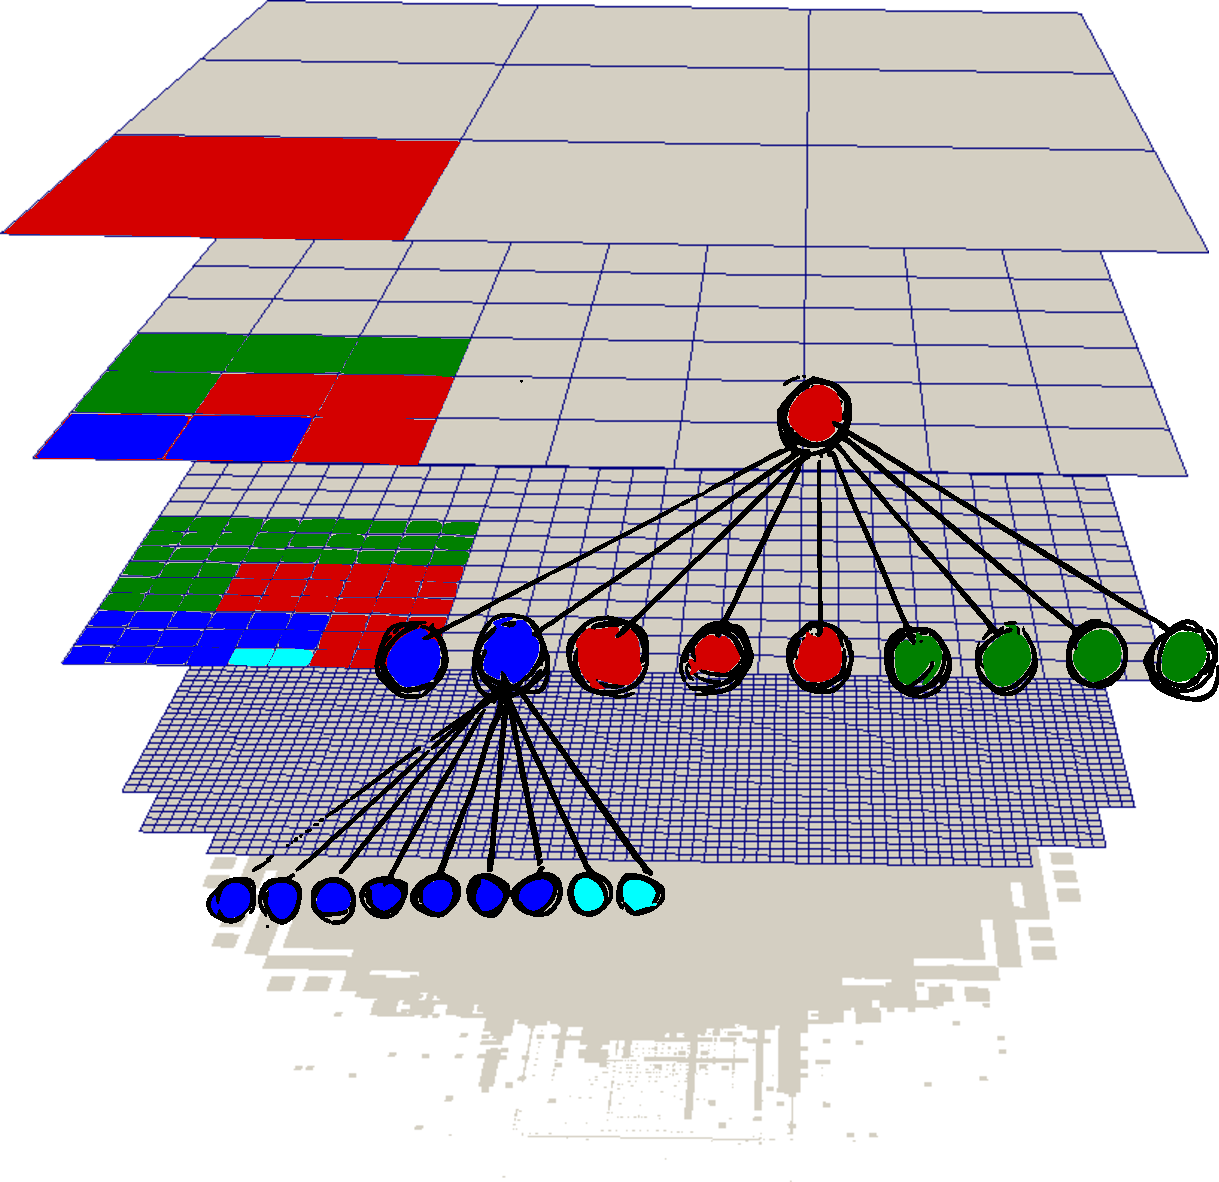
\includegraphics[width=0.5\textwidth]{52_mpi/spacetree-decomposition-top-down.pdf}
\end{center}

\noindent
The picture above details Peano's MPI concept:
The spacetree is top-down split up among the ranks. 
In the present fragment, red is the ``highest'' rank.
When it receives a \texttt{iterate} message from the global master, it also
receives a copy of the master's state as well as a copy of the coarsest cell
belonging to red and its adjacent vertices.
All these data is redundantly stored on the master.
The received state is automatically made the local state.
If you want to do something with the coarsest red cell or the four vertices
belonging to the coarsest level, you can realise 
\begin{code}
void mergeWithWorker(
  exahype::Cell&                               localCell, 
  const exahype::Cell&                         receivedMasterCell,
  const tarch::la::Vector<DIMENSIONS,double>&  cellCentre,
  const tarch::la::Vector<DIMENSIONS,double>&  cellSize,
  int                                          level
);

void mergeWithWorker(
  exahype::Vertex&                             localVertex,
  const exahype::Vertex&                       receivedMasterVertex,
  const tarch::la::Vector<DIMENSIONS,double>&  x,
  const tarch::la::Vector<DIMENSIONS,double>&  h,
  int                                          level
);
\end{code}

\noindent
in one of your mappings. 
Linear algebra codes transfer the residuals or correction values from vertices
through the individual levels.


With all data received, the red node starts to traverse its own tree. 
It recognises that is in turn is the master to two other ranks (green and blue)
and forwards its received state to these guys---as well as the corresponding
cells and vertices on the coarsest common level that the master and its workers
hold redundantly.

Afterwards, red continues to run through its local tree. 
When it starts to ascend through its local tree, it waits for its two workers
(green and dark blue) to terminate and receives from them a state as well as
copies of their coarsest cell plus the adjacent vertices.
This time, the state is not merged into anything automatically. 
However, you can realise the corresponding merge operations to restrict a global
residual value for example.


\subsection{Exchanging boundary data}

Peano realises a non-overlapping domain decomposition on each individual
resolution level.
This means that no cells are held redundantly between two neighbouring ranks on
the same level.
Only the coarsest cell of a rank is also held redundantly by its
master if we compare to \texttt{mergeWithWorker}, e.g.
Boundary data exchange thus exclusively affects vertices. 
It is important to note that all vertices on all levels that are adjacent to
cells of different ranks are exchanged per iteration.
You can switch off the boundary exchange explicitly, but this is subject of
discussion later on as it is a very specific optimisation that is of relevance
only for very few applications.


Mirroring the state behaviour, the code does not literally exchange all
attributes of the vertices.
It exchanges only those attributes of \texttt{Vertex} that are explicitly marked
with \texttt{parallelise} in the DaStGen definition file.  
Yet, exchange means solely that data is sent from one rank to the other and the
other way round---the term does not comprise how data from two vertices held by
two ranks are merged into each other.
Without any merge, copies of vertices along a domain's boundary are sent to all
other ranks per grid sweep, but nothing happens further, i.e.~the exchanged data
is dropped.
To change this, there is the plug-in point

\begin{code}
void prepareSendToNeighbour(
  exahype::Vertex&                             vertex,
  int                                          toRank,
  const tarch::la::Vector<DIMENSIONS,double>&  x,
  const tarch::la::Vector<DIMENSIONS,double>&  h,
  int                                          level
);
\end{code}

\noindent
Whenever a rank finds out that it has just used a vertex for the very last time
throughout a traversal---this happens right after \texttt{touchVertexLastTime}
has been called---and that this vertex is adjacent to multiple ranks and thus
stored on multiple ranks, it calls \texttt{prepareSendToNeighbour} for this
vertex per communication partner \texttt{toRank}.
This operation gives every mapping the opportunity to plug into the send
mechanism.

Peano exchanges its data similar to the Jacobi scheme in linear algebra: 
at the end of an iteration, it sends away copies of vertices. 
Prior to the subsequent traversal, it receives this data and allows the user to
merge it into the local data structures.
For the latter, there is another plug in point:
\begin{code}
void mergeWithNeighbour(
  exahype::Vertex&                              vertex,
  const exahype::Vertex&                        neighbour,
  int                                           fromRank,
  const tarch::la::Vector<DIMENSIONS,double>&   x,
  const tarch::la::Vector<DIMENSIONS,double>&   h,
  int                                           level
);
\end{code}

\noindent
This operation hands you over the local vertex copy as well as the received data
from every other adjacent rank.
While Peano ensures that all grid refinement data, e.g., is kept consistently,
it is your job to ensure that all application-specific data is kept consistent.

A simple matrix-free Jacobi iteration on the vertices thus reads as follows:
\begin{enumerate}
  \item When a vertex is loaded for the very first time throughout a traversal,
  we set its residual to $0$. This happens in \texttt{touchVertexFirstTime()}.
  \item In \texttt{enterCell}, the local residual of this vertex is accumulated.
  \item As soon as we receive \texttt{touchVertexLastTime()} of a particular
  vertex, we know that the code has run through all adjacent cells before. The
  residual hence is complete and we can update the vertex solution according to
  the Jacobi update scheme.
\end{enumerate}

\noindent
This workflow transfers as follows to a distributed memory environment:
\begin{enumerate}
  \item When a vertex is loaded for the very first time throughout a traversal,
  we set its residual to $0$. This happens in \texttt{touchVertexFirstTime()}.
  \item In \texttt{enterCell}, the local residual of this vertex is accumulated.
  \item As soon as we receive \texttt{touchVertexLastTime()} of a particular
  vertex, we know that the code has run through all adjacent cells before {\em
  if the vertex is  a local one}. We can check this with the operation
  \texttt{isAdjacentToRemoteRank()}. The residual hence is complete and we can update the
  vertex solution according to the Jacobi update scheme.
  \item Of a vertex is adjacent to any other rank, we may not update its value.
  We know that this vertex is sent away at the end of the iteration through 
  \texttt{prepareSendToNeighbour}. We do not change any data of the vertex
  herein.
  \item Prior to the next \texttt{touchVertexFirstTime()} on any other rank, we
  know that this rank will receive our local copy of the vertex in
  \texttt{mergeWithNeighbour}. We thus make \linebreak
  \texttt{mergeWithNeighbour} take any
  incoming vertex copy, take the residual from there and merge it into the local
  residual.
  \item If we run into \texttt{touchVertexFirstTime()} for a vertex with
  \texttt{isAdjacentToRemoteRank()}, we know that we didn't update its value yet
  because it had bee incomplete in the previous \texttt{touchVertexLastTime()}
  call. We however know that its residual is accumulated between domain
  boundaries now. We thus update and continue with the standard \linebreak
  \texttt{touchVertexFirstTime()}.
\end{enumerate}



\subsection{Exchanging boundary data on the heap}

Different to the vertex boundaries, heap data is not automatically exchanged by
Peano's MPI. 
There are different variants how to manage heaps. 
The simplest one is to instruct Peano via the communication specification that
you use a heap and want the code to exchange heap data along the domain
boundaries.
For this, your mappings have to define a communication specification
that sets the third flag to \texttt{true}.
By default, the generated specification uses \texttt{false}. 
Setting the flag instructs the Peano kernel that you want to use
heaps for boundary data exchange as well.
\begin{code}
peano::CommunicationSpecification  
myMapping::communicationSpecification() { 
  return peano::CommunicationSpecification( ...,...,true );
}
\end{code}

\noindent
The flag tells Peano that heaps are used for communication and that you want the
kernel to synchronise all communication channels. 
Notably, the kernel now ensures that all data is received before you start a new
traversal, and it releases data sent via nonblocking MPI automatically once a
traversal terminates.

\begin{remark}
If you fuse multiple mappings onto one adapter and one of the mappings specifies
\texttt{true} while all other mappings do not set this flag, then Peano will
administer the heap, i.e.~the single \texttt{true} dominates the behaviour.
However, you'll receive warnings that the various communication specifications
are inconsistent with each other. To remove those warnings, ensure that all
mappings either set the flag or not.
\end{remark}


Yet, no actual bundary data is sent and received yet. 
If you want to exchange data through a boundary vertex, you have to do so
explicitly in \texttt{prepareSendToNeighbour}.
Please note that Peano's heap has specialised operations for this:
\begin{code}
void myMapping::prepareSendToNeighbour(
  particles::pidt::Vertex&                      vertex,
  int                                           toRank,
  const tarch::la::Vector<DIMENSIONS,double>&   x,
  const tarch::la::Vector<DIMENSIONS,double>&   h,
  int                                           level
) {
  MyHeap::getInstance().sendData(
    index-of-heap-entry,
    toRank,
    x,
    level,
    peano::heap::MessageType::NeighbourCommunication
  );
}
\end{code}

\noindent
The counterpart has to be realised in \texttt{mergeWithNeighbour}.
Peano takes care that all data is exchanged in the right order as efficiently as
possible.

\begin{remark}
You are responsible to ensure that each heap send operation has a
corresponding receive on the other side for exactly the same vertex in the next
grid sweep.
As the data exchange is distributed between two iterations, you might decide to
implement the receive in a different mapping.
However, you have to ensure that each send is mapped by exactly one receive on
the vertex counterpart.
\end{remark}

\noindent
Instead of relying on the \texttt{true} flag in the specification, you can
decide to administer all the heaps yourself. 
If you do this, you have instruct the heap in \texttt{beginIteration} that you
start to exchange data (via the operation \texttt{startToSendBoundaryData}),
while you tell Peano in \texttt{endIteration} that this exchange has finished
through \texttt{finishedToSendBoundaryData}.


Most codes work fine with an automated heap data exchange administration. 
However, with a manual instruction, you are allowed to send out data in one
iteration and receive it a couple of iterations later.
The manual exchange operations of the heap class ensure that all data is
exchanged in the right order. 
You have to ensure that the number of sends and receives as well as the ordering
which vertex sends and receives match.
If you allow Peano to squeeze one or more traversals in-between a send and the
subsequent receive, you release pressure from MPI: 
Peano deploys all heap data exchange to non-blocking sends and receives.
It now has more time to transfer the actual data.
 


\subsection{Exchanging heap data vertically (in-sync)}

The previous paragraphs discussed the exchange of heap data between different
adjacent partitions. 
We call this horizontal data exchange (within a level).
If you want to exchange data between masters and workers or the other way round,
you can still rely on the heap's send and receive operations.
However, the data transfer semantics change.


Exchange between masters and workers is synchronous.
We do not send out data in one iteration and receive it in the subsequent
iteration, but we want to send out data when we descend into a worker tree node,
and this data has to be received just before this worker actually starts its
traversal.
To trigger this behaviour, you can still use the heap's send and receive, but
you have to pass 
\texttt{peano::heap::MessageType::MasterWorkerCommunication} as last argument.
This tells Peano that you want synchronous data exchange.


The heaps still work with non-blocking data transfers of MPI.
This helps to avoid blocking buffers and, thus, deadlocks. 
Therefore, we also have to tell the heap when you start a synchronous data
exchange and when you finish it.
For this, there are routines \texttt{startToSendSynchronousData} and
\texttt{finishedToSendSynchronousData} offered by every heap.


\begin{remark}
While Peano is built to use localised point-to-point messages only, you may want
to exchange data between any two ranks. The heaps allow you to do so---either
similar to a boundary data exchange where sent data is to be received in the
subsequent grid sweep or similar to a master-worker communication where sent
data is received right away.
\end{remark}


\begin{remark}
(Dynamic) Load balancing transfers data from one MPI rank to another one
synchronously: either from a master to a new worker when we split up a partition
or from a worker to a master if we merge two partitions into one subdomain. If
you have to transfer heap data here, you can apply the same pattern you've used
for master-worker data transfer. However, you should use the flag  
\texttt{peano::heap::MessageType::ForkOrJoinCommunication} rather than 
\texttt{peano::heap::MessageType::MasterWorkerCommunication} in your send and
receive calls.
Peano then uses different MPI tags and thus ensures that master-worker messages and fork-join
transfer data is not mixed up.
For the fork/join data, the heap requires no notification that data exchange
starts or stops; the kernel internally knows this already.
\end{remark}


\subsection{Running global steps on all ranks and manually broadcast
information from the global master}

Not all algorithms decompose exclusively into a sequence of grid sweeps. 
Software with explicit matrix assembly, e.g., maps the matrix assembly itself,
all plotting, postprocessing, time stepping and so forth onto grid traversals.
The global solve (via PETSc, e.g.) however is a plain function call per MPI
rank.
We may introduce an adapter/mapping for this, switch to this adapter on the
global master and trigger the adapter iterate on the global master.
The corresponding mapping for such a global step then however is almost trivial:
it does something in \texttt{beginIteration} or \texttt{endIteration} while the
actual grid traversal remains empty. 
Though such a translation of global steps into grid sweeps follows the pure
Peano philosophy, it is neither convenient to program nor is it efficient.
It is a waste of resources as the whole grid is piped through
the traversal once for the global step.


As alternative to the sketched variant, Peano's repository offers a
routine \texttt{runGlobalStep} while each worker implements a
\texttt{runGlobalStep}, too. 
To let all non-idle MPI ranks do one thing at a time, you implement the
following steps:

\begin{enumerate}
  \item Inside your global master's code, i.e.~somewhere within
  \texttt{runAsMaster}, you call \texttt{runGlobalStep} on your repository.
  \item You implement \texttt{runGlobalStep} in your runner. The repository call
  invokes this routine on all non-idle workers.
  \item If you want the global master to run through your runner's
  \texttt{runGlobalStep}, too, you have to call this one manually.
\end{enumerate}

The term non-idle in the paragraphs above refers to Peano's load balancing.
MPI's load balancing oracles can decide which and how many ranks at any time are
participating in the computation.
The load balancing may decide that some MPI ranks are not used at a certain
time.
They remain idle;
and they are then not affected by the global step.


\texttt{runGlobalStep}'s signature is empty.
We can start one routine simultaneously on all non-idle ranks, but we can not
natively hand over data.
However, you are always free to send data via MPI yourself. 
There are a few remarks on consider however and there are some support routines
that might be of value:

\begin{itemize}
  \item You can rely on plain MPI to exchange data. However, you can also model
  your messages with DaStGen which is convenient as DaStGen equips the modelled
  data structure with MPI send and receive commands.
  \item It is simple to receive data from and send data to the global master on
  the worker rankas, as the master's global rank number is available through the
  \texttt{Node}.
  \item The node pool offer a broadcast operation to send any message modelled
  with DaStGen out to all non-idle ranks.
  \item Alternatively (if you prefer to work with plain MPI, e.g.), it offers a
  query to ask for each rank whether it is idle or not.
  \item The node pool allows you to obtain an MPI tag. It is highly recommended
  to make your own global communication run through MPI tags of their own. This
  way, you ensure that your data sends and receives to not interfer with other
  MPI messages of Peano still pending in the network.
\end{itemize}

\noindent
Via the exchange of MPI messages within \texttt{runGlobalStep}, you can
implement different steps: you can basically send around an integer or enum
which triggers different behaviour on the ranks.
Below is an example of a manual global data distribution that relies on plain
MPI. 
As highlighted, modelling the messages with DaStGen yields shorter and more
elegant code:

\begin{code}
  const int myTag = tarch::parallel::Node::getInstance().reserveFreeTag(...);

  double myValue = 2; // you might want to use a DaStGen class instead of primitive types

  if (tarch::parallel::Node::getInstance().isGlobalMaster()) {
     double receivedValue;
     for (int rank=1; rank<tarch::parallel::Node::getInstance().getNumberOfNodes(); rank++) {
       if ( !tarch::parallel::NodePool::getInstance().isIdleNode(rank) ) {
         MPI_Recv( &receivedValue, 1, MPI_DOUBLE, rank, myTag,
           tarch::parallel::Node::getInstance().getCommunicator(),
           MPI_STATUS_IGNORE ); // would be a simple method invocation with DaStGen objects 
         myValue += receivedValue;
       }
     }
  }
  else {
    MPI_Send( &myValue, 1, MPI_DOUBLE, tarch::parallel::Node::getGlobalMasterRank(),
      myMessageTagUseForTheReduction, tarch::parallel::Node::getInstance().getCommunicator() );
  }

  tarch::parallel::Node::getInstance().releaseTag(myTag);
\end{code}


\subsection{Wrap-up, preparatory work and per-sweep pre- and postprocessing
on a worker}

In large codes, there's often a need to plug into the creation of a rank
(everytime it is used by the load balancing to handle a part of the grid) or to
run some pre- and postprocessing steps per grid traversal. 
To do so, you may add code to the pregenerated \texttt{RunnerParallelWorker.cpp}
file that even contains, if created by the development toolkit, some remarks
where to add source code.


\subsection{Further MPI remarks}

\begin{itemize}
  \item If you couple Peano with another component using MPI, and the two codes
  shall not interfer with collectives, you can change Peano's {\textbf
  communicator}.
  For this, have a look into \texttt{tarch::parallel::Node}. All Peano kernel
  routines ask the \texttt{Node} class which communicator to use. So change it
  there and you switch Peano to a different communicator.
  \item Peano uses various MPI {\textbf tags} to exchange data. Most Peano
  components grab a tag from a central data base and then work with this tag,
  i.e.~the tags are hidden from the user. If you want to exchange your own data
  with MPI commands and want to ensure not to interfer with any Peano messages,
  use the static operation \texttt{reserveFreeTag} from \linebreak
  \texttt{tarch::parallel::Node} in the system setup to reserve a tag for your
  own purposes that then exclusive to you.
  \item If you want to exchange data along the master-worker {\textbf topology} or
  with the {\textbf global rank}, it is best to ask the
  texttt{tarch::parallel::NodePool} for the right ranks. Usually, rank 0 is the
  global master. However, Peano can be reconfigured to change this
  behaviour---which is particularly useful if you couple the AMR framework with
  some other codes.
\end{itemize}



\subsection*{Further reading}

\begin{itemize}
  \item T. Weinzierl: 
  {\em The {P}eano software---parallel,
   automaton-based, dynamically adaptive grid traversals}.
  arXiv:1506.04496
  \item 
  T. Weinzierl and M. Mehl: {\em Peano---A Traversal and Storage Scheme for
Octree-Like Adaptive Cartesian Multiscale Grids}.
In R. Tuminaro, M. Benzi, X.-C. Cai, I. Duff, H. Elman, R. Freund, K. Jordan, T.
Kelley, D. Keyes, M. Kilmer, S. Leyffer, T. Manteuffel, S. McCormick, D.
Silvester, H. Walker, C. Woodward and I. Yavneh (ed.), SIAM Journal on
Scientific Computing, Volume 33{\textbf(5)} of Special Section: 2010 Copper Mountain
Conference, pp.~2732--2760, 2011.
  \item 
H.-J. Bungartz, W. Eckhardt, T. Weinzierl and C. Zenger: {\em A Precompiler to
Reduce the Memory Footprint of Multiscale PDE Solvers in C++}.
In P.M.A. Sloot (ed.), Future Generation Computer Systems, Volume 26{\textbf (1)},
pp.~175--182. Elsevier, 2010.
  \item 
T. Weinzierl: {\em A Framework for Parallel PDE Solvers on Multiscale Adaptive
Cartesian Grids}.
Dissertation, Institut f\"ur Informatik, Technische Universit\"at M\"unchen. Verlag Dr. Hut, M\"unchen, 2009.
    \item 
H.-J. Bungartz, M. Mehl, T. Weinzierl and W. Eckhardt: {\em DaStGen - A Data
Structure Generator for Parallel C++ HPC Software}.
In Bubak, van Albada, Sloot and Dongarra (ed.), ICCS 2008: Advancing Science
through Computation, Part III, Volume 5103 of Lecture Notes in Computer Science,
pp.~213--222. Springer-Verlag, Heidelberg, Berlin, June 2008.
\end{itemize}
